% Copyright 2011, Piotr Jakubowski

\chapter{Project definition}
  This chapter aims to state the scope of the project. Moreover, I would like to draw an outline of expected output and point out challenges that I would have to face during the development.
  
  \section{Scope of the project}
  As stated in the introduction, generation of administration panel seems to be an actual problem. Therefore, my aim is to develop a plugin or rather a gem\footnote{TODO: More on gems in chapter bla bla bla} for Ruby language that would provide functionality of administration panel generation for Ruby on Rails application. 
  
  One of the first assumptions was that the installation of the administration panel should be effortless and should not require any changes to the code of application. Moreover, the administration panel should detect changes to business models "on-the-fly" and should adjust to reflect those changes in the panel without need of running any generators or other scripts.
  
  The functionality of the administration panel would consist of:
  \begin{itemize}
	  \item Listing all of business models in the application.
	  \item For particular model listing all of the records.
	  \item Creation and edition of records using automatically generated forms.
	  \item Deletion of records.
	  \item Proper handling of associations between models.
	  \item Configuration of the panel regarding which models or model fields should be visible.
	\end{itemize}
	
	\section{Project outline}
	The project would be developed for test application that would be a simple blog system. The functionality of the test application would be a subject of adjustments in order to check and prove appropriate functioning of the plugin. 
	
	To start with, test application would allow following actions:
	\begin{itemize}
	  \item Add, edit, list and delete posts
	  \item Add, edit, list and delete categories
    \item Assign posts to appropriate categories
	\end{itemize}
	
  Target functionality of plugin has been stated in previous section. Mockups of user interface of the plugin are depicted in figures  \ref{mockup01}, \ref{mockup02} and \ref{mockup03}
	
	\begin{figure}[hbt!]
		\begin{center}
			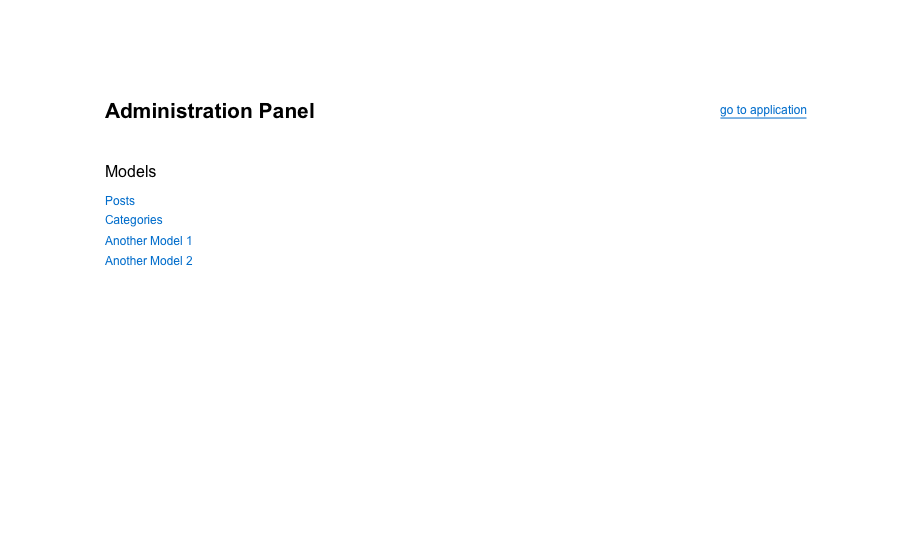
\includegraphics[width=\linewidth]{images/chapter02/mockup01.png}
			\caption{Mockup of dashboard page of the plugin}
			\label{mockup01}
		\end{center}
	\end{figure}
	
	\begin{figure}[hbt!]
		\begin{center}
			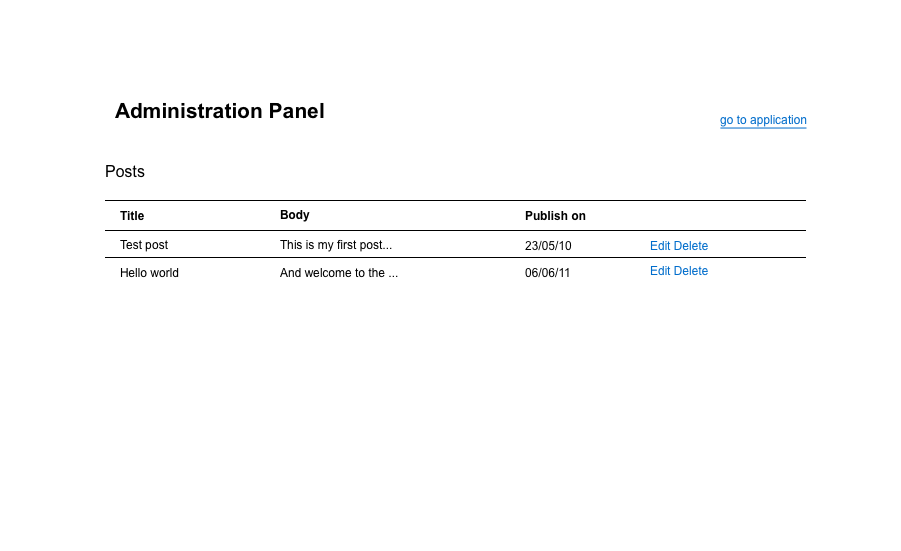
\includegraphics[width=\linewidth]{images/chapter02/mockup02.png}
			\caption{Mockup of page for listing records of given model}
			\label{mockup02}
		\end{center}
	\end{figure}
	
	\begin{figure}[hbt!]
		\begin{center}
			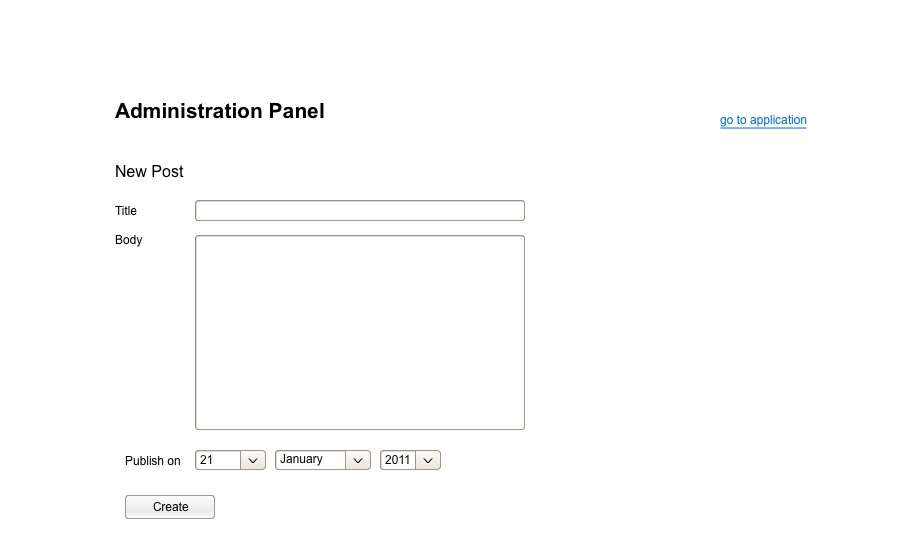
\includegraphics[width=\linewidth]{images/chapter02/mockup03.png}
			\caption{Example page for creation or edition of model record}
			\label{mockup03}
		\end{center}
	\end{figure}
	
	\section{Anticipated challenges}
	The challenge that is most striking while approaching this project is the fact that the solution has to be universal and totally independent of any domain specific workarounds. As a plugin, it has to be usable for all or at least majority of web applications. Therefore, it is necessary to take into consideration all kinds of association between models and all types of fields that may appear in those models. Moreover, I would have to watch out not to violate any business logic that some developer put in his models or not to introduce data inconsistency. Fortunately, well-design systems would rather fail raisin an exception than allow to perform some illegal action on models.
	
	Furthermore, it seems like a lot of code in this project would need to figure out actions itself during the runtime basing on what kind of code would be in the application. In order to make that plugin functional, it would be necessary to dive into and make use of meta-programming, which may not be as easy to use, clear and readable. Fortunately, Ruby from its nature of being a dynamic language allows many meta-programming actions and provides developers with very pleasant reflection API.
	
	Hopefully, those challenges would get overcome during design and development of the project in order to produce plugin that would make life of web programmers slightly easier.
	
	